% Options for packages loaded elsewhere
% Options for packages loaded elsewhere
\PassOptionsToPackage{unicode}{hyperref}
\PassOptionsToPackage{hyphens}{url}
\PassOptionsToPackage{dvipsnames,svgnames,x11names}{xcolor}
%
\documentclass[
  letterpaper,
  DIV=11,
  numbers=noendperiod]{scrartcl}
\usepackage{xcolor}
\usepackage[margin=2.5cm]{geometry}
\usepackage{amsmath,amssymb}
\setcounter{secnumdepth}{5}
\usepackage{iftex}
\ifPDFTeX
  \usepackage[T1]{fontenc}
  \usepackage[utf8]{inputenc}
  \usepackage{textcomp} % provide euro and other symbols
\else % if luatex or xetex
  \usepackage{unicode-math} % this also loads fontspec
  \defaultfontfeatures{Scale=MatchLowercase}
  \defaultfontfeatures[\rmfamily]{Ligatures=TeX,Scale=1}
\fi
\usepackage{lmodern}
\ifPDFTeX\else
  % xetex/luatex font selection
\fi
% Use upquote if available, for straight quotes in verbatim environments
\IfFileExists{upquote.sty}{\usepackage{upquote}}{}
\IfFileExists{microtype.sty}{% use microtype if available
  \usepackage[]{microtype}
  \UseMicrotypeSet[protrusion]{basicmath} % disable protrusion for tt fonts
}{}
\makeatletter
\@ifundefined{KOMAClassName}{% if non-KOMA class
  \IfFileExists{parskip.sty}{%
    \usepackage{parskip}
  }{% else
    \setlength{\parindent}{0pt}
    \setlength{\parskip}{6pt plus 2pt minus 1pt}}
}{% if KOMA class
  \KOMAoptions{parskip=half}}
\makeatother
% Make \paragraph and \subparagraph free-standing
\makeatletter
\ifx\paragraph\undefined\else
  \let\oldparagraph\paragraph
  \renewcommand{\paragraph}{
    \@ifstar
      \xxxParagraphStar
      \xxxParagraphNoStar
  }
  \newcommand{\xxxParagraphStar}[1]{\oldparagraph*{#1}\mbox{}}
  \newcommand{\xxxParagraphNoStar}[1]{\oldparagraph{#1}\mbox{}}
\fi
\ifx\subparagraph\undefined\else
  \let\oldsubparagraph\subparagraph
  \renewcommand{\subparagraph}{
    \@ifstar
      \xxxSubParagraphStar
      \xxxSubParagraphNoStar
  }
  \newcommand{\xxxSubParagraphStar}[1]{\oldsubparagraph*{#1}\mbox{}}
  \newcommand{\xxxSubParagraphNoStar}[1]{\oldsubparagraph{#1}\mbox{}}
\fi
\makeatother


\usepackage{longtable,booktabs,array}
\newcounter{none} % for unnumbered tables
\usepackage{calc} % for calculating minipage widths
% Correct order of tables after \paragraph or \subparagraph
\usepackage{etoolbox}
\makeatletter
\patchcmd\longtable{\par}{\if@noskipsec\mbox{}\fi\par}{}{}
\makeatother
% Allow footnotes in longtable head/foot
\IfFileExists{footnotehyper.sty}{\usepackage{footnotehyper}}{\usepackage{footnote}}
\makesavenoteenv{longtable}
\usepackage{graphicx}
\makeatletter
\newsavebox\pandoc@box
\newcommand*\pandocbounded[1]{% scales image to fit in text height/width
  \sbox\pandoc@box{#1}%
  \Gscale@div\@tempa{\textheight}{\dimexpr\ht\pandoc@box+\dp\pandoc@box\relax}%
  \Gscale@div\@tempb{\linewidth}{\wd\pandoc@box}%
  \ifdim\@tempb\p@<\@tempa\p@\let\@tempa\@tempb\fi% select the smaller of both
  \ifdim\@tempa\p@<\p@\scalebox{\@tempa}{\usebox\pandoc@box}%
  \else\usebox{\pandoc@box}%
  \fi%
}
% Set default figure placement to htbp
\def\fps@figure{htbp}
\makeatother





\setlength{\emergencystretch}{3em} % prevent overfull lines

\providecommand{\tightlist}{%
  \setlength{\itemsep}{0pt}\setlength{\parskip}{0pt}}



 


\KOMAoption{captions}{tableheading}
\makeatletter
\@ifpackageloaded{caption}{}{\usepackage{caption}}
\AtBeginDocument{%
\ifdefined\contentsname
  \renewcommand*\contentsname{Table of contents}
\else
  \newcommand\contentsname{Table of contents}
\fi
\ifdefined\listfigurename
  \renewcommand*\listfigurename{List of Figures}
\else
  \newcommand\listfigurename{List of Figures}
\fi
\ifdefined\listtablename
  \renewcommand*\listtablename{List of Tables}
\else
  \newcommand\listtablename{List of Tables}
\fi
\ifdefined\figurename
  \renewcommand*\figurename{Figure}
\else
  \newcommand\figurename{Figure}
\fi
\ifdefined\tablename
  \renewcommand*\tablename{Table}
\else
  \newcommand\tablename{Table}
\fi
}
\@ifpackageloaded{float}{}{\usepackage{float}}
\floatstyle{ruled}
\@ifundefined{c@chapter}{\newfloat{codelisting}{h}{lop}}{\newfloat{codelisting}{h}{lop}[chapter]}
\floatname{codelisting}{Listing}
\newcommand*\listoflistings{\listof{codelisting}{List of Listings}}
\makeatother
\makeatletter
\makeatother
\makeatletter
\@ifpackageloaded{caption}{}{\usepackage{caption}}
\@ifpackageloaded{subcaption}{}{\usepackage{subcaption}}
\makeatother
\usepackage{bookmark}
\IfFileExists{xurl.sty}{\usepackage{xurl}}{} % add URL line breaks if available
\urlstyle{same}
\hypersetup{
  pdftitle={Forecasting Industrial Production Using FRED-MD Data},
  pdfauthor={Aruzhan Zhumazhan and Salima Myrzabek},
  colorlinks=true,
  linkcolor={blue},
  filecolor={Maroon},
  citecolor={Blue},
  urlcolor={Blue},
  pdfcreator={LaTeX via pandoc}}


\title{Forecasting Industrial Production Using FRED-MD Data}
\usepackage{etoolbox}
\makeatletter
\providecommand{\subtitle}[1]{% add subtitle to \maketitle
  \apptocmd{\@title}{\par {\large #1 \par}}{}{}
}
\makeatother
\subtitle{Big Data Applications --- June 2026}
\author{Aruzhan Zhumazhan and Salima Myrzabek}
\date{}
\begin{document}
\maketitle


\section{Data Description}\label{data-description}

The dataset used in this project is the FRED-MD database, a large
monthly macroeconomic dataset containing more than 100 U.S.
macroeconomic and financial variables. The dataset includes indicators
related to industrial production, employment, prices, interest rates,
money, credit, and financial markets.

The target variable is \texttt{INDPRO}, the Industrial Production Index.
It measures real output in the manufacturing, mining, and utilities
sectors of the U.S. economy. Since industrial production in levels
usually follows a trend over time, the target variable is transformed
into a stationary growth-rate series using the first difference of the
logarithm:

\[
w_t = \log(INDPRO_t) - \log(INDPRO_{t-1})
\]

This transformed variable represents the monthly growth rate of
industrial production and is used as the dependent variable in the
forecasting models.

\section{Data Cleaning and
Preprocessing}\label{data-cleaning-and-preprocessing}

\subsection{COVID-19 Period Removal}\label{covid-19-period-removal}

Observations from January 2020 to July 2020 are removed from the
dataset. This period contains large pandemic-related shocks and
structural breaks. These observations are not representative of normal
macroeconomic dynamics and may distort model estimation and forecast
evaluation.

\subsection{Outlier Treatment}\label{outlier-treatment}

Outliers are removed using a robust interquartile range rule. For each
numeric variable, values more than ten times the interquartile range
away from the median are replaced by missing values. This conservative
threshold removes only extremely abnormal observations while keeping
regular macroeconomic variation in the dataset.

\subsection{Missing Value Treatment}\label{missing-value-treatment}

Missing values are handled using a sequential procedure. First, linear
interpolation is applied. Then, remaining missing values are filled
using forward fill and backward fill. Finally, any remaining missing
observations are replaced by the mean of the corresponding variable.

\begin{longtable}[]{@{}rll@{}}
\caption{Missing value treatment procedure.}\tabularnewline
\toprule\noalign{}
Step & Method & Purpose \\
\midrule\noalign{}
\endfirsthead
\toprule\noalign{}
Step & Method & Purpose \\
\midrule\noalign{}
\endhead
\bottomrule\noalign{}
\endlastfoot
1 & Linear interpolation & Fill gaps between observed values \\
2 & Forward fill & Use the last available observation \\
3 & Backward fill & Use the next available observation \\
4 & Mean imputation & Replace any remaining missing values \\
\end{longtable}

\subsection{Transformation to
Stationarity}\label{transformation-to-stationarity}

The raw \texttt{INDPRO} series is transformed into the log-difference
series \texttt{w}. This removes the long-run trend and makes the target
variable more suitable for time-series forecasting.

\begin{figure}[H]

{\centering \pandocbounded{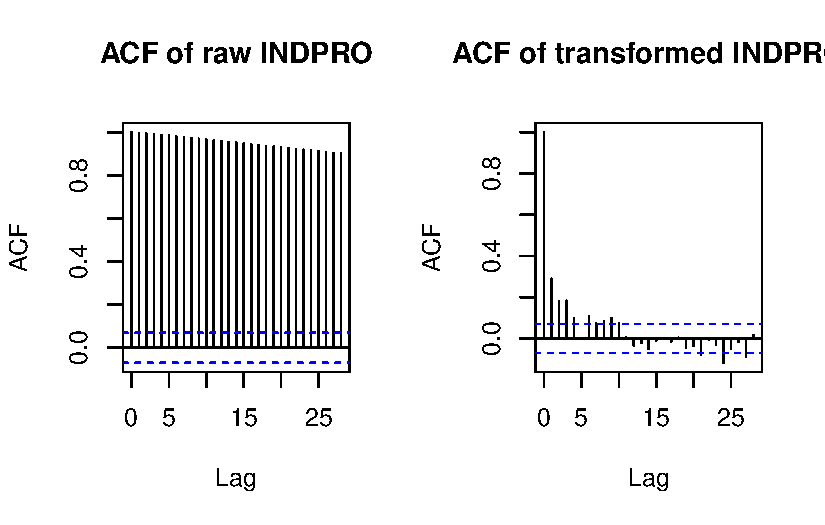
\includegraphics[keepaspectratio]{forecast_files/figure-pdf/acf-plot-1.pdf}}

}

\caption{ACF comparison of raw and transformed INDPRO.}

\end{figure}%

\subsection{Standardization}\label{standardization}

All predictors are centered and standardized before estimation. The
target variable is also standardized. This is important because the
predictors are measured on different scales. Standardization improves
numerical stability and makes penalized regression methods such as Ridge
and Lasso more reliable.

\section{Training and Test Sample}\label{training-and-test-sample}

The initial training sample contains the first 524 observations after
cleaning and transformation. The remaining observations are used for
out-of-sample forecast evaluation. Forecasts are produced using an
expanding-window procedure. In each step, the model is re-estimated
using all data available up to that point, and a one-step-ahead forecast
is produced for the next period.

\section{Forecasting Methods}\label{forecasting-methods}

\subsection{AR(1)}\label{ar1}

The AR(1) model uses only the first lag of the target variable:

\[
y_t = \alpha + \beta y_{t-1} + \varepsilon_t
\]

The number of lags is set to one because the project focuses on
one-step-ahead forecasting and uses a simple autoregressive benchmark.

\subsection{Random Walk}\label{random-walk}

A random walk is a simple benchmark where the best forecast for the next
period is the current value. In this project, the main simple benchmark
is the AR(1) model, which is a more flexible version because it
estimates the persistence parameter instead of fixing it equal to one.

\subsection{OLS}\label{ols}

The OLS model uses all lagged standardized predictors from the FRED-MD
dataset:

\[
y_t = \alpha + X_{t-1}\beta + \varepsilon_t
\]

This model can use many macroeconomic variables, but it may overfit
because the number of predictors is large.

\subsection{Ridge Regression}\label{ridge-regression}

Ridge regression adds an L2 penalty to the regression coefficients:

\[
\min_\beta \|y - X\beta\|^2 + \lambda \|\beta\|^2
\]

The penalty parameter is selected using the Bayesian Information
Criterion over a grid of candidate values.

\subsection{Lasso Regression}\label{lasso-regression}

Lasso regression adds an L1 penalty:

\[
\min_\beta \|y - X\beta\|^2 + \lambda \|\beta\|_1
\]

This method can shrink some coefficients exactly to zero and therefore
performs variable selection. In the code, the penalty parameter is
selected using the BIC criterion.

\subsection{Principal Component
Regression}\label{principal-component-regression}

Principal Component Regression reduces the high-dimensional predictor
matrix to a smaller set of common factors. These factors are extracted
using singular value decomposition and then used in the forecasting
regression. The number of principal components is selected using BIC.

\section{Results}\label{results}

\subsection{Principal Component
Selection}\label{principal-component-selection}

The scree plot shows how much variation is explained by the first
principal components.

\begin{figure}[H]

{\centering \pandocbounded{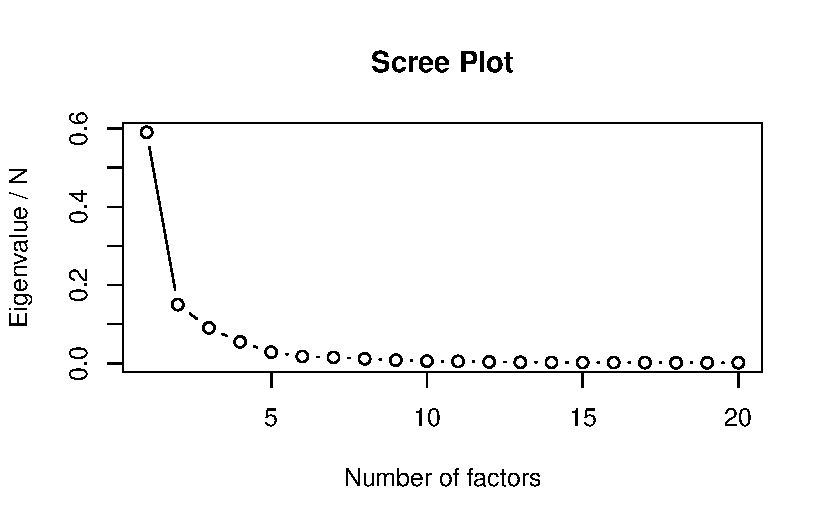
\includegraphics[keepaspectratio]{forecast_files/figure-pdf/scree-plot-1.pdf}}

}

\caption{Scree plot of the first 20 principal components.}

\end{figure}%

The next figure shows the BIC values for different numbers of principal
components. The number of factors with the lowest BIC is selected for
the PCA regression.

\begin{figure}[H]

{\centering \pandocbounded{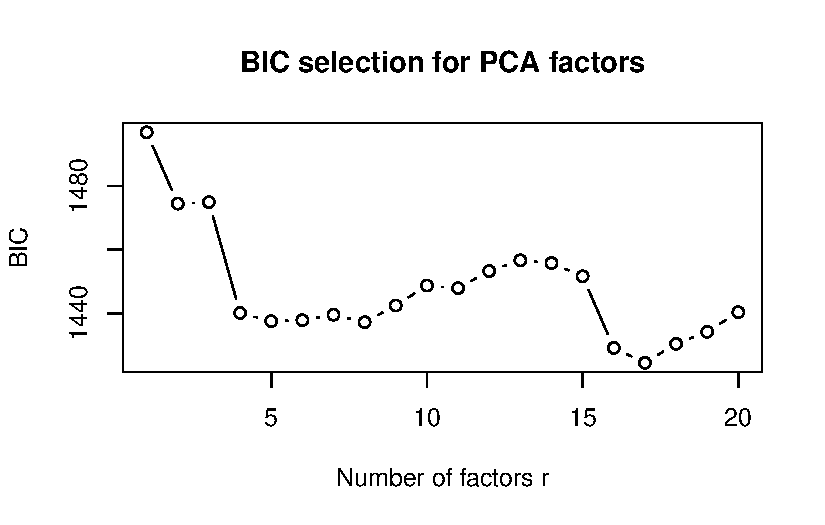
\includegraphics[keepaspectratio]{forecast_files/figure-pdf/bic-plot-1.pdf}}

}

\caption{BIC selection for the number of PCA factors.}

\end{figure}%

\subsection{One-Step-Ahead Forecasts}\label{one-step-ahead-forecasts}

\begin{longtable}[]{@{}lrr@{}}
\caption{One-step-ahead forecasts for transformed INDPRO growth and
INDPRO level.}\tabularnewline
\toprule\noalign{}
Model & Forecast\_w & Forecast\_INDPRO\_level \\
\midrule\noalign{}
\endfirsthead
\toprule\noalign{}
Model & Forecast\_w & Forecast\_INDPRO\_level \\
\midrule\noalign{}
\endhead
\bottomrule\noalign{}
\endlastfoot
AR(1) & 0.002005 & 90.81925 \\
OLS & 0.003173 & 90.92537 \\
Ridge BIC & 0.002161 & 90.83336 \\
Lasso BIC & 0.002784 & 90.89002 \\
PCA Regression & 0.001044 & 90.73194 \\
\end{longtable}

\subsection{Root Mean Squared Errors}\label{root-mean-squared-errors}

Forecast accuracy is evaluated using Root Mean Squared Error:

\[
RMSE = \sqrt{\frac{1}{H}\sum_{t=1}^{H}(y_t - \hat{y}_t)^2}
\]

A lower RMSE means better out-of-sample forecasting performance.

\begin{longtable}[]{@{}llr@{}}
\caption{RMSE comparison for transformed INDPRO growth.}\tabularnewline
\toprule\noalign{}
& Model & RMSE\_w \\
\midrule\noalign{}
\endfirsthead
\toprule\noalign{}
& Model & RMSE\_w \\
\midrule\noalign{}
\endhead
\bottomrule\noalign{}
\endlastfoot
3 & Ridge BIC & 0.007751 \\
4 & Lasso BIC & 0.008093 \\
5 & PCA Regression & 0.008378 \\
1 & AR(1) & 0.008491 \\
2 & OLS & 0.012639 \\
\end{longtable}

\begin{longtable}[]{@{}llr@{}}
\caption{RMSE comparison for INDPRO levels.}\tabularnewline
\toprule\noalign{}
& Model & RMSE\_INDPRO \\
\midrule\noalign{}
\endfirsthead
\toprule\noalign{}
& Model & RMSE\_INDPRO \\
\midrule\noalign{}
\endhead
\bottomrule\noalign{}
\endlastfoot
3 & Ridge BIC & 0.754754 \\
4 & Lasso BIC & 0.786053 \\
5 & PCA Regression & 0.813868 \\
1 & AR(1) & 0.825792 \\
2 & OLS & 1.255582 \\
\end{longtable}

\subsection{Forecast Comparison
Graphs}\label{forecast-comparison-graphs}

The following graph compares actual and forecasted values for the
transformed target variable.

\begin{figure}[H]

{\centering \pandocbounded{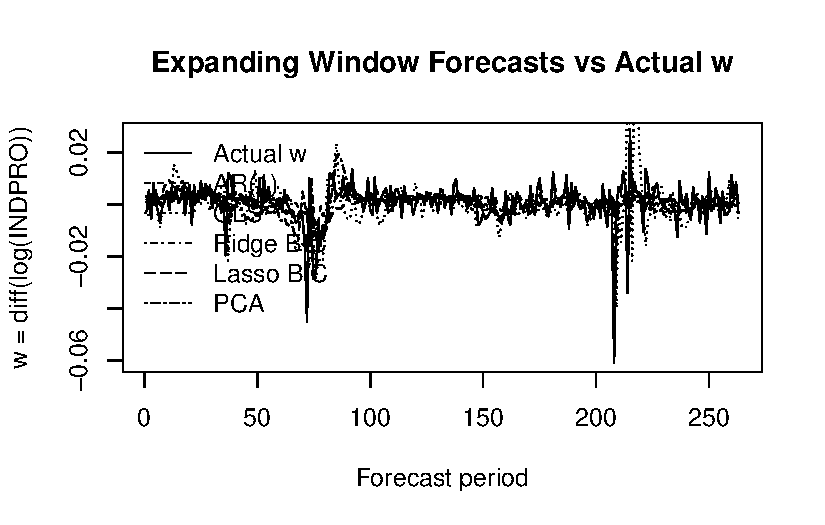
\includegraphics[keepaspectratio]{forecast_files/figure-pdf/forecast-w-plot-1.pdf}}

}

\caption{Expanding-window forecasts compared with actual transformed
INDPRO growth.}

\end{figure}%

The next graph compares the forecasts after converting them back to the
INDPRO level.

\begin{figure}[H]

{\centering \pandocbounded{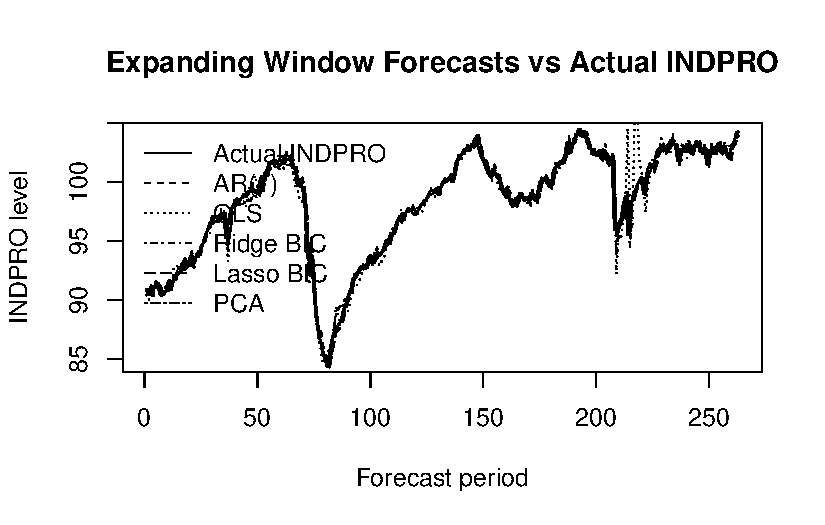
\includegraphics[keepaspectratio]{forecast_files/figure-pdf/forecast-level-plot-1.pdf}}

}

\caption{Expanding-window forecasts compared with actual INDPRO level.}

\end{figure}%

\section{Discussion of Results}\label{discussion-of-results}

The results compare simple autoregressive forecasting, unrestricted
regression, regularized regression, and factor-based regression. The
best method is the one with the lowest RMSE in the out-of-sample
evaluation. Regularized methods such as Ridge and Lasso are expected to
perform well in this setting because the dataset contains many
correlated macroeconomic predictors. These methods reduce overfitting by
shrinking coefficient estimates.

Principal Component Regression is also useful because it summarizes the
information in many predictors into a smaller number of common factors.
This can improve forecast stability when many variables share similar
macroeconomic movements.

OLS may perform worse because it estimates many coefficients without
regularization. In high-dimensional macroeconomic data, this can lead to
unstable estimates and poor out-of-sample forecasts. The AR(1) benchmark
is simpler and often competitive because industrial production growth is
persistent, but it does not use the additional information contained in
the FRED-MD predictors.

Overall, the preferred model is the one ranked first in the RMSE table.
This method provides the most accurate out-of-sample forecasts for
industrial production in this forecasting exercise.

\section{Code Submission}\label{code-submission}

The full R code is submitted separately in the accompanying
\texttt{forecast.R} file.




\end{document}
